\subsection{Runtime Adaptation}
\label{sec:adaptation}

\begin{figure}
  \centering
  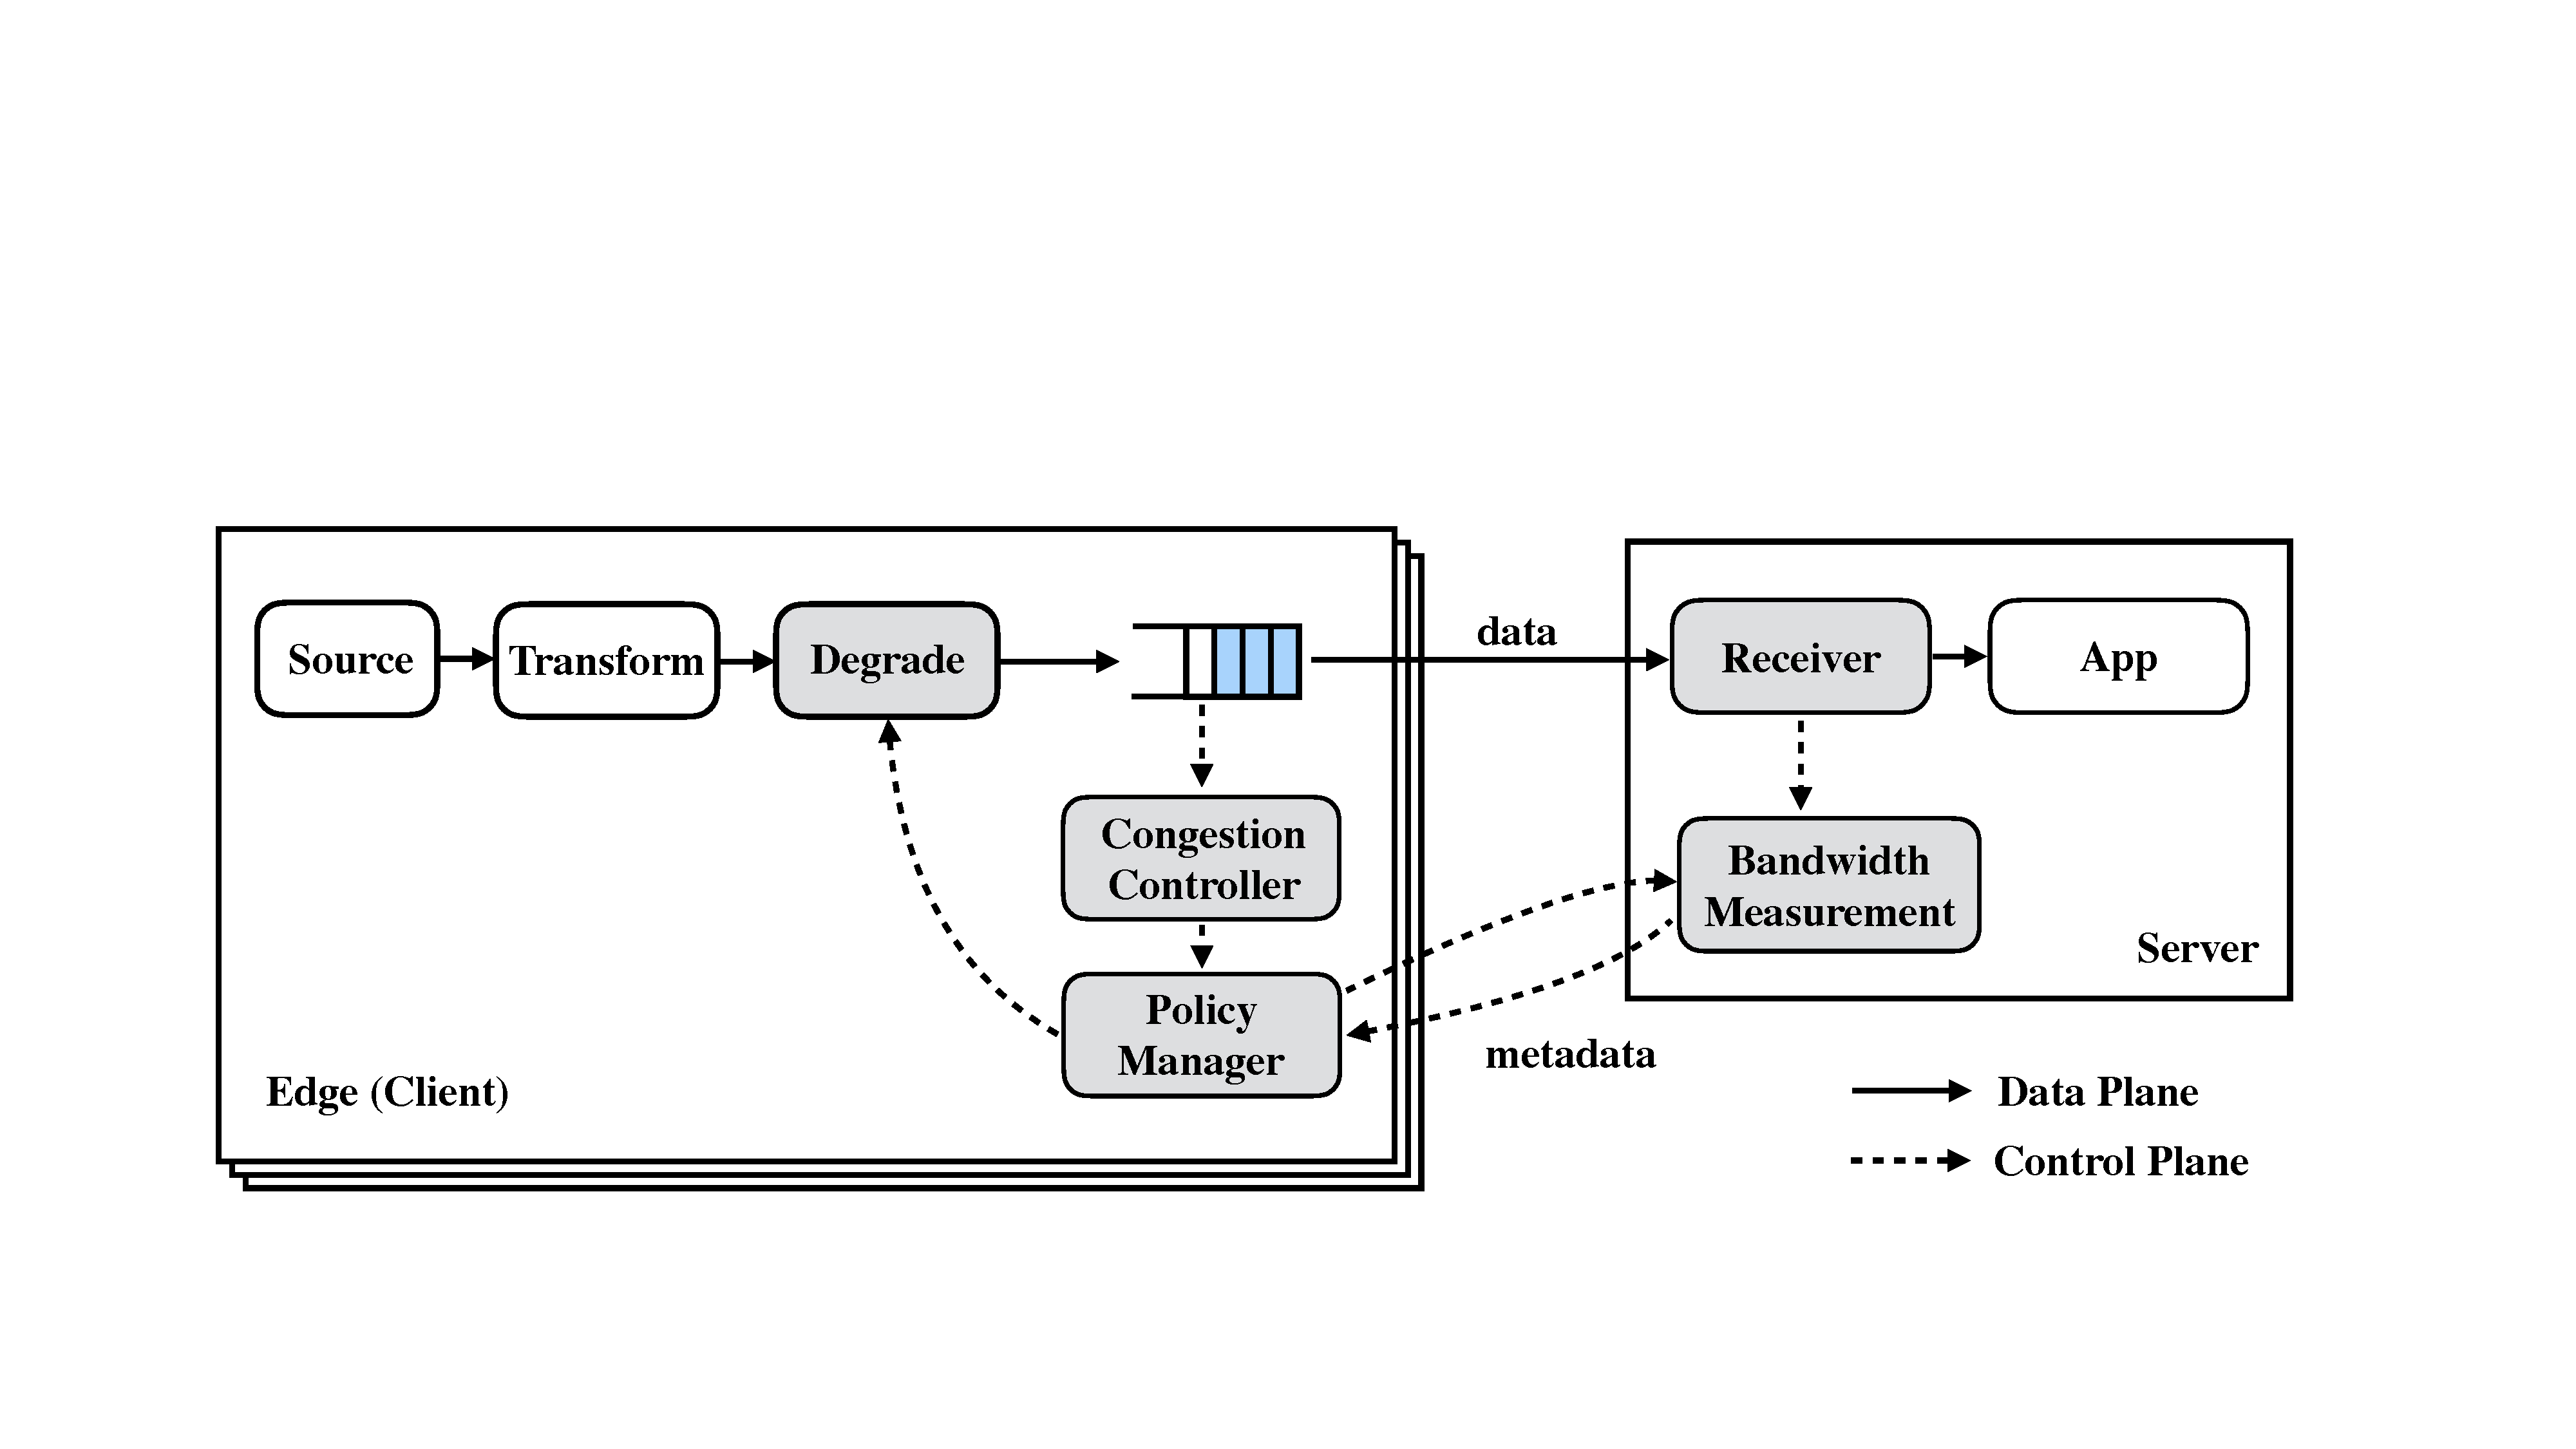
\includegraphics[width=\linewidth]{figures/runtime.pdf}
  \caption{Runtime adaptation system architecture. The grey components are what
    \sysname{} provides.}
  \label{fig:runtime}
\end{figure}

At runtime, the user program is automatically converted to a client half and
server half; and \sysname{} abstracts the communication as well as rate
adaptation. \autoref{fig:runtime} shows our runtime architecture.

\para{Object-level queue:} The queue bridges data generation and
the network capacity. It transmits data as fast as the network can handle and
detects congestion when the queue grows.

\para{Congestion controller:} Our first prototype used the queue length as a
signal for congestions, this turns out to be a bad match as the degradation
operation may change object arrival rate (e.g.\,lower frame rate for video). Our
next version uses data size, but it also leads to long latency when the
degradation changes individual object size (e.g.\,lower resolution). Our current
design uses an adaptive size: given current configuration and the profile, the
queue learns the desired data generation rate (bps), and with a user configured
latency, the queue derive the congestion watermark.

\para{Bandwidth Measurement:} The receiver delivers the received data to
application. In the meantime, it measures the effective throughput between each
client-server pair as an indication of current bandwidth~\cite{iperf}. To avoid
spikes in the bandwidth measurement, exponential smoothing is employed. While
the receiver performs bandwidth measurement every second, it does not send the
information back to each client.  avoid unnecessary communication, the client
requests the measurement only when congestion is detected.

\para{Policy Manager:} Upon receiving signals from congestion controller, it
performs an RPC request to the server for current bandwidth measurement. With
the learned profile, it determines the degradation level and start the actual
degradation strategy. The bandwidth specification in the learned profile is the
required bandwidth, the policy manager usually takes a conservative approach:
using a constant rate ALPHA to adjust the available bandwidth. When the
congestion is resolved, the policy manager gradually reduce the degradation
level (additive increase phase).

\para{Degrade:} The actual degradation operation is rather simple. Operators
based on the \texttt{maybe} API supports a \texttt{set} function that would
change the internals of the operator. The \texttt{set} function is invoked when
degradation is needed.

%% {Interaction with TCP:} Our runtime system follow the tuning guide
%% \cite{tierney2001tcp} to adjust the send buffer.

%%% Local Variables:
%%% mode: latex
%%% TeX-master: "sigcomm2017"
%%% End:
